We will now turn our attention to pruning methods. Pruning is concerned with removing specific branches to improve some metrics measuring
the tree's performance. First we will analyze the functionality of the provided \emph{pruning\_example} function.
We will conclude with a discussion of more general pruning.



\lstset{language=matlab}

\begin{lstlisting}
function pruning_example(x,y)
    
% x: noSamples x 45 (as returned by loaddata)
% y: noSamples x 1 (as returned by loaddata)

tree = classregtree(x,y,'method','classification','categorical',1:45,'minparent',1,'prune','off');
view(tree);
[cost,s,nodes,bestLevel] = test(tree,'cross',x,y);
[cost2,s2,nodes2,bestLevel2] = test(tree,'resubstitution');

prunedTree = prune(tree,'level',bestLevel);
prunedTree2 = prune(tree,'level',bestLevel2);

\end{lstlisting}




The \emph{classregtree()} function takes, in the examples, matrix x, as well as the label matrix y.
It then creates a classification tree that predicts the labels using the columns of the examples matrix.\\
The parameter 'categorical' tells the function to treat the columns of x (the attributes) as unordered categorical variables
such that each attribute takes on one of a discrete, limited and fixed set of values (here '1' or '0').\\
The parameter 'minparent = 1' dictates that impure nodes that contain 1 or more examples should be split.\\
Since a node that contains 1 example is by definition pure,
this really means that impure nodes that contain 2 or more examples should be split.\\
The parameters 'prune = off' dictates that there should be no pruning of the tree.

This function is actually different than the way we build trees because our model consists of six trees that each classify a given
example.
We then extract a label from these six classifications from the trees, with various methods described in the ambiguity section.
The \emph{classregtree()} function works differently and builds one tree,
where the leaf nodes are non-binary and instead take on one of the 6 emotion values.
For the purpose of this discussion, pruning,
this will not matter as it can be applied to each of our trees to yield better classification rates.

The \emph{test()} function removes increasingly more nodes from the tree, in iterations called 'levels'.
I could not find online how they define a level and how they decide which nodes to remove,
but the general pattern is to prune from bottom to top increasingly.
I believe they used a combination of the depth of a terminal node and the number of examples that lie at this node.
At each of these levels, it computes a cost of the tree, calculated as the parameters 'cross' and 'resubstitution' dictate it.
If 'cross' is the parameter, the examples and labels are fed to the function as well, which are used to carry out a 10-fold
cross-validation. When creating the 10 folds, it applies stratification such that labels are present in roughly equal proportions
in each fold. I could not find which metric they use to extract a cost from the cross-validation, but I assume it is something
like the average error rate.\\
If 'substitution' is the parameter, the cost of the tree is computed as the sum over all of this level's terminal
nodes of a node's estimated probability times its cost.
A node's cost is the sum of the misclassification costs of the examples at that node.
Again, I could not find how they define misclassification costs.
Note that the resubstitution cost is computed from the same sample that was used to train the tree as opposed to the cross-validation
cost method.\\
The method returns three vectors, each of size equal to the number of levels of pruning. The first vector, cost, contains a cost
of the tree for each level of pruning. The second vector contains the standard error of each cost value from the first vector.
Again, it is not clear how they compute the standard error of the cost. The third vector simply lists the number of nodes at each
level of pruning. Lastly, the method returns the level as the one that produces the smallest tree that is within one standard
error of the minimum-cost subtree.

The \emph{prune()} function prunes a tree to the given desired level, and returns the pruned tree.
Here it is called twice, once with the best level as per the 'substitution' method and one as per the 'cross' method.
Below, you will find the diagrams returns by the code snippet.



\begin{figure}[h]
    \caption{Clean dataset}
    \begin{center}
  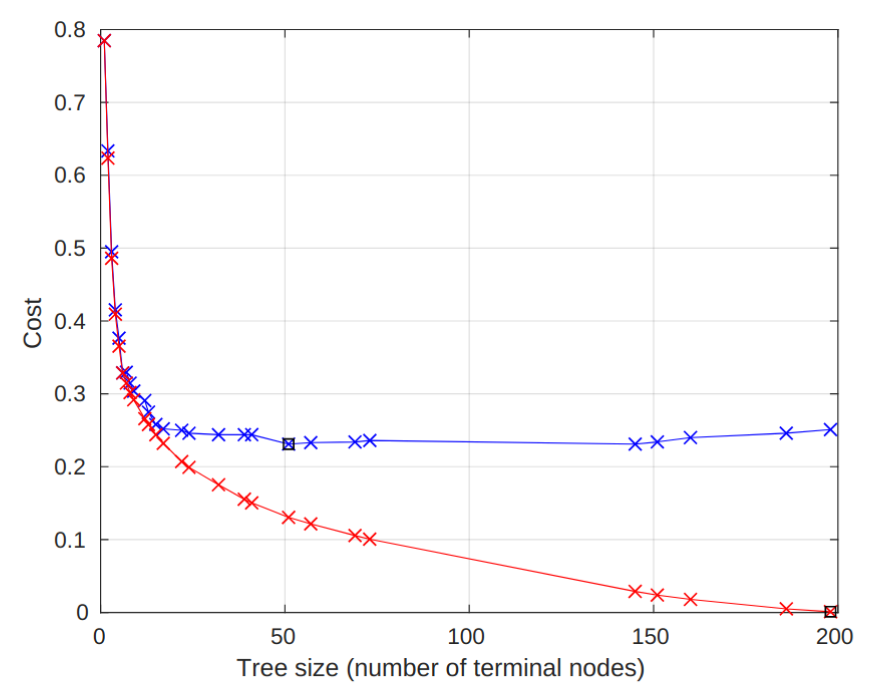
\includegraphics[scale = 0.40]{graphs/clean_dataset/clean_pruning.png}
 \end{center}
  \end{figure}


 \begin{figure}[h]
    \begin{center}
    \caption{Noisy dataset}
  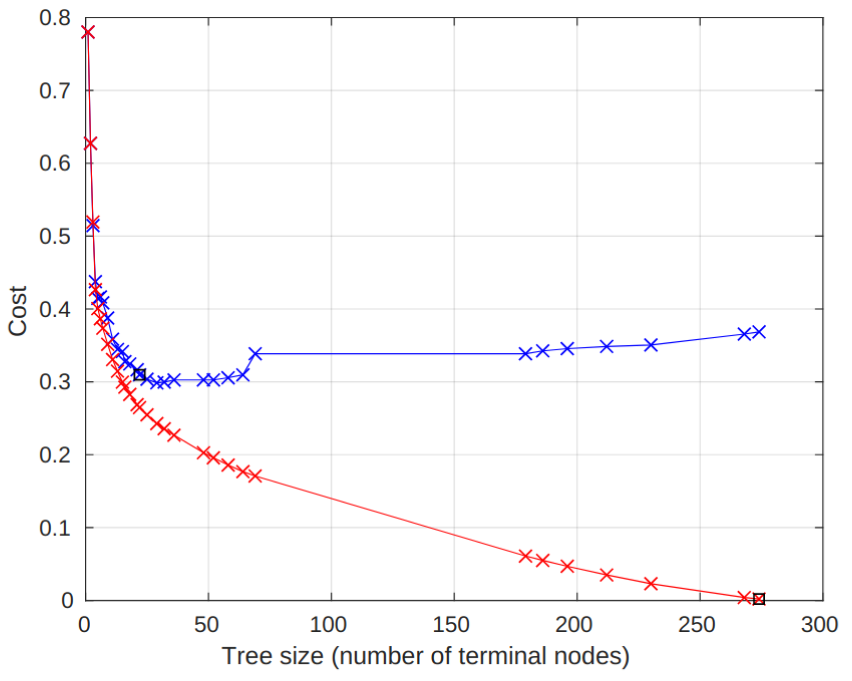
\includegraphics[scale = 0.40]{graphs/noisy_dataset/noisy_pruning.png} 
 \end{center}

  \end{figure}

\newpage

The data used to generate this graph comes from \emph{test()} function,
taken from each level, and simply plots the number of terminal nodes at this level versus
the cost of the tree obtained by pruning to this level.
In red, you will find the results of the 'resubstitution' method and thus in blue, the results of the 'cross' method.
As you can see, the 'resubstitution' method yields much lower costs at almost every number of terminal.
This is explained as the 'resubstitution' evaluates its misclassification costs on the very data that was used to train
the trees, which is sure to yield few misclassifications as opposed to cross-validation, which evaluates misclassification costs
using the holdout fold that was not used to train the tree.
Furthermore, the 'resubstitution' method costs stricly decrease as the number of terminal nodes increases.
This results in the best level to prune at being '0' for both datasets and thus no pruning at all occurs.\\
The 'cross' method however yields a best level that prunes the trees significantly, especially with the noisy dataset.
This indicates that there is some level of overfitting present in our tree. This ties in quite well with our previous discussions
where we expressed our view that emotions with few data points would introduce overfitting.
